\subsection{Part A: Simulation results}
\label{sec:results-a}

\subsubsection{Perception envelope}

The filter's accuracy is governed by range through the $\alpha r^2/s$ measurement noise model. As the vehicle is about 5~m from the dock, the fused noise floor is approximately 0.11~m and the filter's health node reports \textsc{degraded} throughout the run. At 2.2~m, the floor drops to about 0.02~m and the filter is \textsc{healthy} for the 92\% of the run (with median position standard deviation of 0.018~m). During this range, the velocity state is able to track teh true dock velocity, with an amplitude ration of 0.85 and correlation of 0.89, see Figure~\ref{fig:vel-check}. However, on the opposite extreme, marker visibility collapses at contact range. Binning the fine-alignment health by ground-truth range shows 84\% to 100\% healthy beyond 5~cm from the entry, but only 21\% inside it. This blackout is produced by the marker corners overflowing the camera field of view (FoV). The size-graded layout behaves as intended here since teh detection hands over from the outer large markers (201 and 202) to the interior and eye level markers as each size class overflows in turn. The blackout only begins where even the smallest pair no longer fits in the frame, so the measured envelope is therefore reliable from roughly 2.5~m to 0.05~m.

\begin{figure}[H]
    \centering
    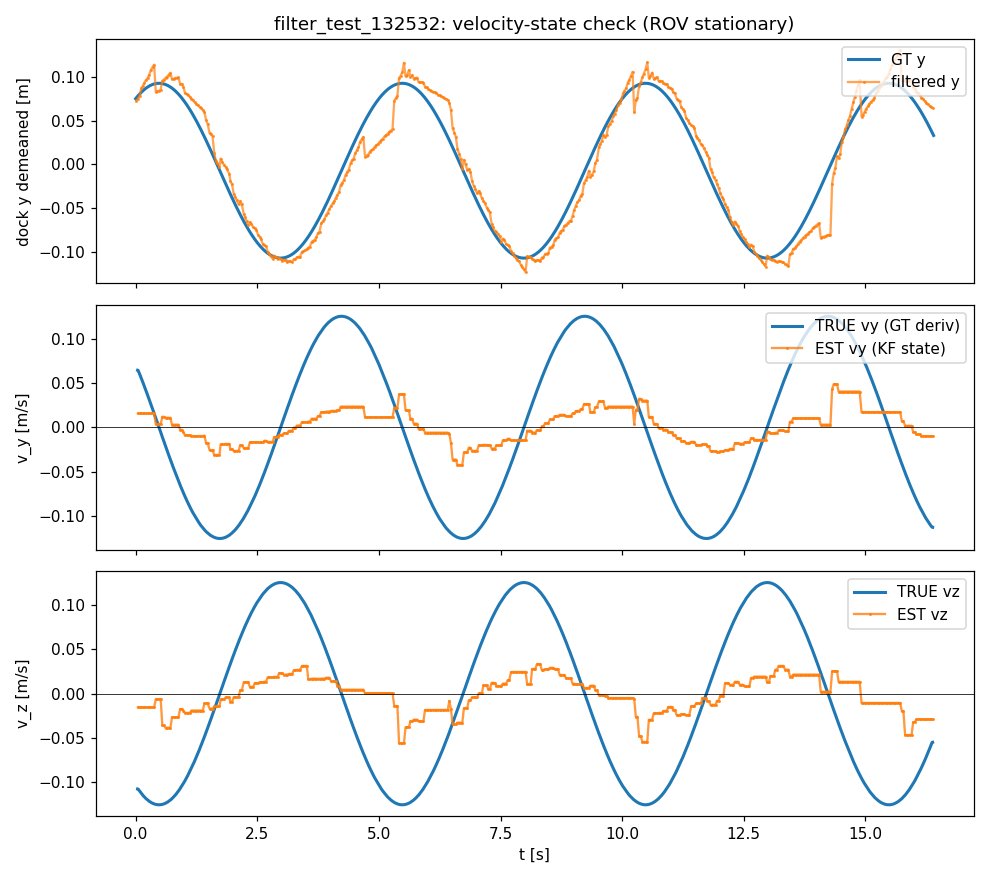
\includegraphics[width=0.85\textwidth]{Figures/vel_check.png}
    \caption{Dock velocity estimation with the vehicle stationary at 2.2~m
        (5~s sway period). Top: filtered dock sway against ground truth.
        Middle and bottom: the filter velocity state against the ground-truth
        dock velocity in sway and heave.}
    \label{fig:vel-check}
\end{figure}

\subsubsection{Docking demonstration}

Against the nominal 18~s, 0.1~m orbital sway, the system docks autonomously end to end (Figure~\ref{fig:trajectory}). The vehicle engages to coarse at $t{+}4$~s, hands off to fine alignment at $t{+}15$~s, and is seated and docked at $t{+}26$~s with no demotions. It latches 7 to 8~cm from the entry and comes to rest 4~cm in front of the dock plane. The trajectory shows the two-stage structure directly, in which the coarse phase closes 4~m to the standoff point, then fine alignment performs the lateral correction onto the moving entry axis before the final advance. The range curves plateau briefly at 1~m in both trials. This is the hold at the coarse standoff, where the vehicle decelerates under the distance-gated surge cap, overshoots the standoff point slightly and settles back while the debounced handoff gate clears. In the sway trial, the dock's own motion during the hold adds a small range wobble on top. The static-dock sanity trial is overlaid for comparison, and it follows a nearly straight approach and seats at 19~s. The cost of the 18~s sway is therefore the lateral correction and roughly seven additional seconds, without a qualitative change in behaviour. Both trials, and every sweep trial below, ran the full perception pipeline in the loop with no ground-truth input to the vehicle.

\begin{figure}[H]
    \centering
    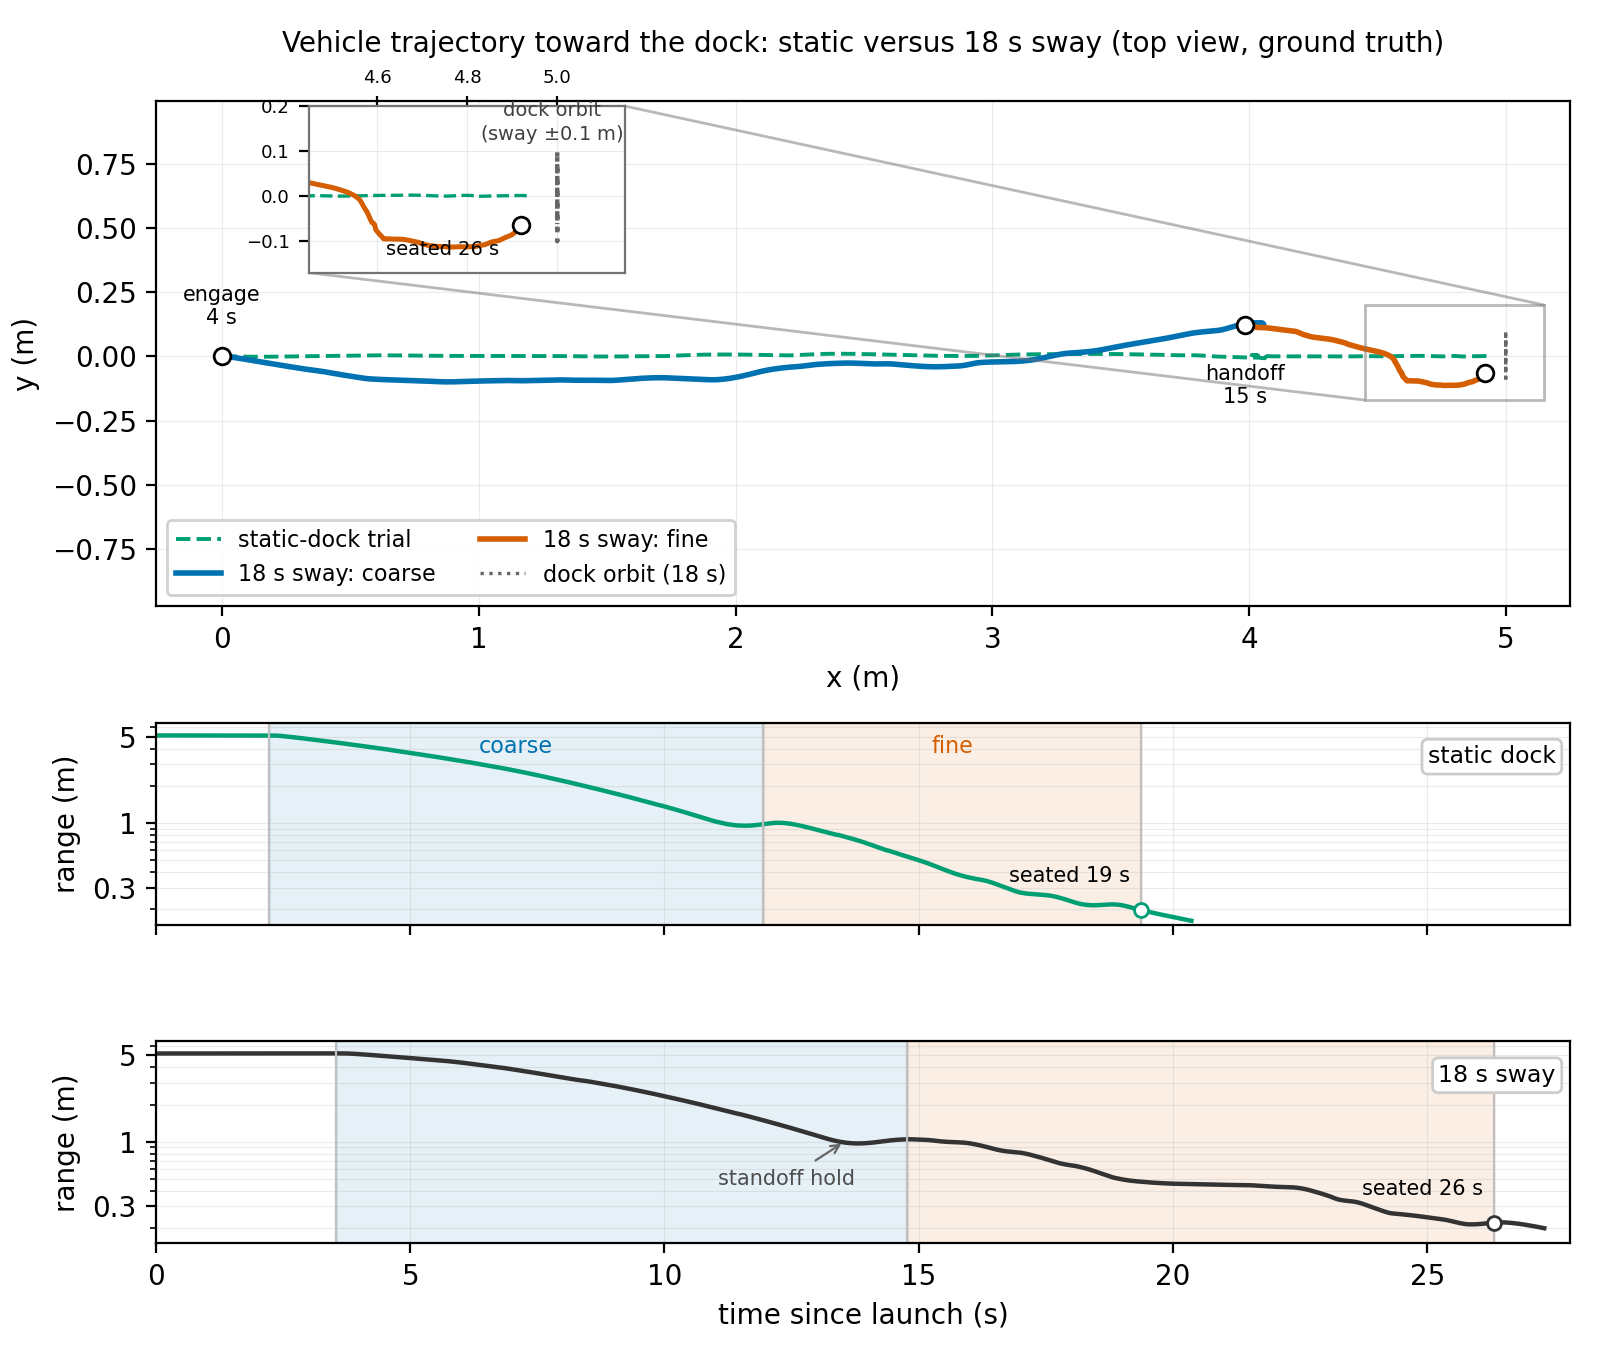
\includegraphics[width=0.95\textwidth]{Figures/rov_trajectory.png}
    \caption{The demonstration trial (18~s sway period) against the
        static-dock sanity trial. Top: ground-truth vehicle trajectories in
        the horizontal plane, coloured by mission phase, with the terminal
        region magnified in the inset. Bottom: range to the dock origin on a
        logarithmic scale, one panel per trial with its phase timing shaded.
        The plateau at 1~m is the hold at the coarse standoff.}
    \label{fig:trajectory}
\end{figure}

\subsubsection{Docking envelope versus sway period}

Figure~\ref{fig:pdock} shows the result of the sweep ($n{=}3$ per cell, contact-censored scoring). The baseline (static filter, no feedforward) docks in every trial at every period in the raw scoring, and cleanly down to 8~s. At 6~s, two of the three trials brush the aperture boundary at low speed (0.03 to 0.06~m/s) before latching. The method (constant-velocity filter with feedforward) matches the baseline down to 12~s, degrades at 10~s (one pre-latch contact), and fails at 8~s and 6~s. Its single raw success at 8~s was contact-assisted.

\begin{figure}[H]
    \centering
    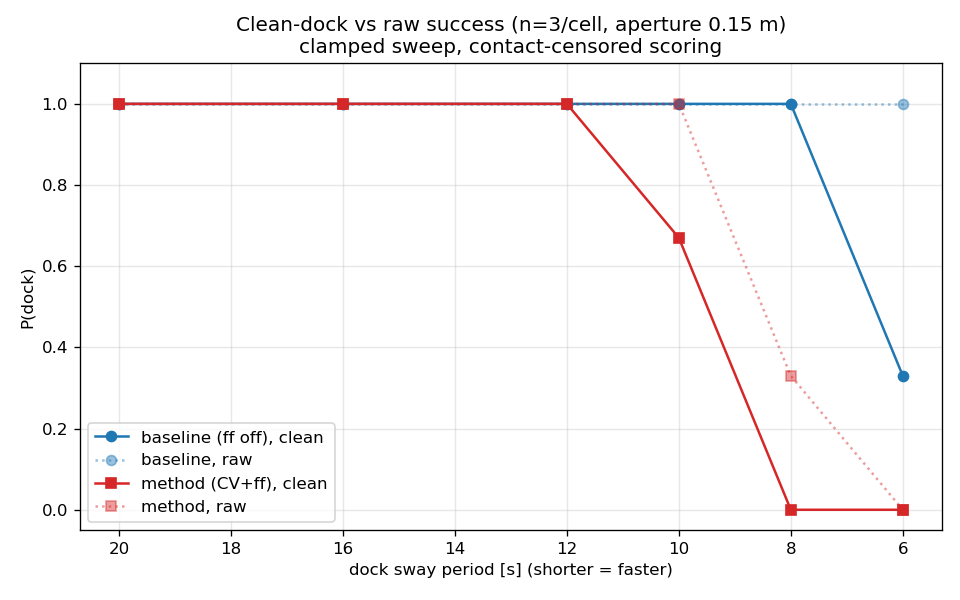
\includegraphics[width=0.8\textwidth]{Figures/clean_pdock.png}
    \caption{Docking success versus sway period under raw (dotted) and
        contact-censored clean (solid) scoring.}
    \label{fig:pdock}
\end{figure}

In the operational terms of Section~\ref{sec:method-sim}, each period cell maps to a sea state and a dock depth. The mean NSW sea (8~s period, 1.6~m significant height) forces a 0.1~m sway on a dock near 33~m depth, which the baseline handles cleanly. The 6~s wind-sea cell corresponds to a shallow dock near 19~m in the same sea, where the baseline still docks in every trial under raw scoring. The longer-period cells correspond to deeper moorings reached only by swell, where both configurations succeed. The measured envelope therefore covers moored docks across typical continental-shelf operating depths, with the residual risk concentrated in shallow, short-period deployments. Notably, the method's cliff at 8 to 10~s sits at the region's mean wave period, which is why the baseline's immunity matters operationally.

Clean insertions cross the entry plane 0.003 to 0.05~m off axis at 0.06 to 0.11~m/s closing speed, and all observed contacts occur below 0.06~m/s. These figures form the interface requirement for a capture mechanism, where a funnel with a capture radius of at least 0.15~m and a tolerance for approximately 0.1~m/s closing speed captures everything the baseline delivers down to 8~s periods.

\subsubsection{Failure analysis: ego-motion instability of the velocity estimator}

The method's fast-period failures share a single mechanism. The dock measurement is reconstructed in the world frame through the transform of a moving camera, so a fraction of the vehicle's own motion leaks into the measured dock position. This leakage is correlated with the vehicle state, which violates the filter's white-noise assumption. The static filter has no velocity state, so it absorbs the leakage as position noise and remains faithful (the estimated sway amplitude is 0.7 to 0.9 times the truth in all baseline runs). The constant-velocity filter instead integrates the leakage into a phantom dock velocity and extrapolates it. The estimated amplitude reaches 2.4 to 5 times the truth in successful method runs, and 18 to 52 times in the failures, where the estimate has decoupled from the real dock (a correlation of 0.00 with the true dock, while the estimate's excess motion correlates at 0.88 with the vehicle's own position). The feedforward then closes the loop by injecting the phantom velocity directly into the command. With the identified plant lag of approximately 240~ms, the loop gain crosses unity between the 10~s and 8~s periods, which is where the measured cliff sits.

Figure~\ref{fig:trajectory-failure} shows the mechanism in a single failed trial at the 8~s period. In the tracking segments, the estimated dock sway already exceeds the true amplitude while the vehicle overshoots further still. When the resulting misalignment costs marker visibility and the measurements are gated out, the constant-velocity model dead-reckons on the phantom velocity. The estimated dock position ramps to a full metre off (ten times the true amplitude, with the velocity clamp active) while the vehicle follows it. Reacquisition then snaps the estimate back, the supervisor demotes, and the cycle repeats without ever seating.

\begin{figure}[H]
    \centering
    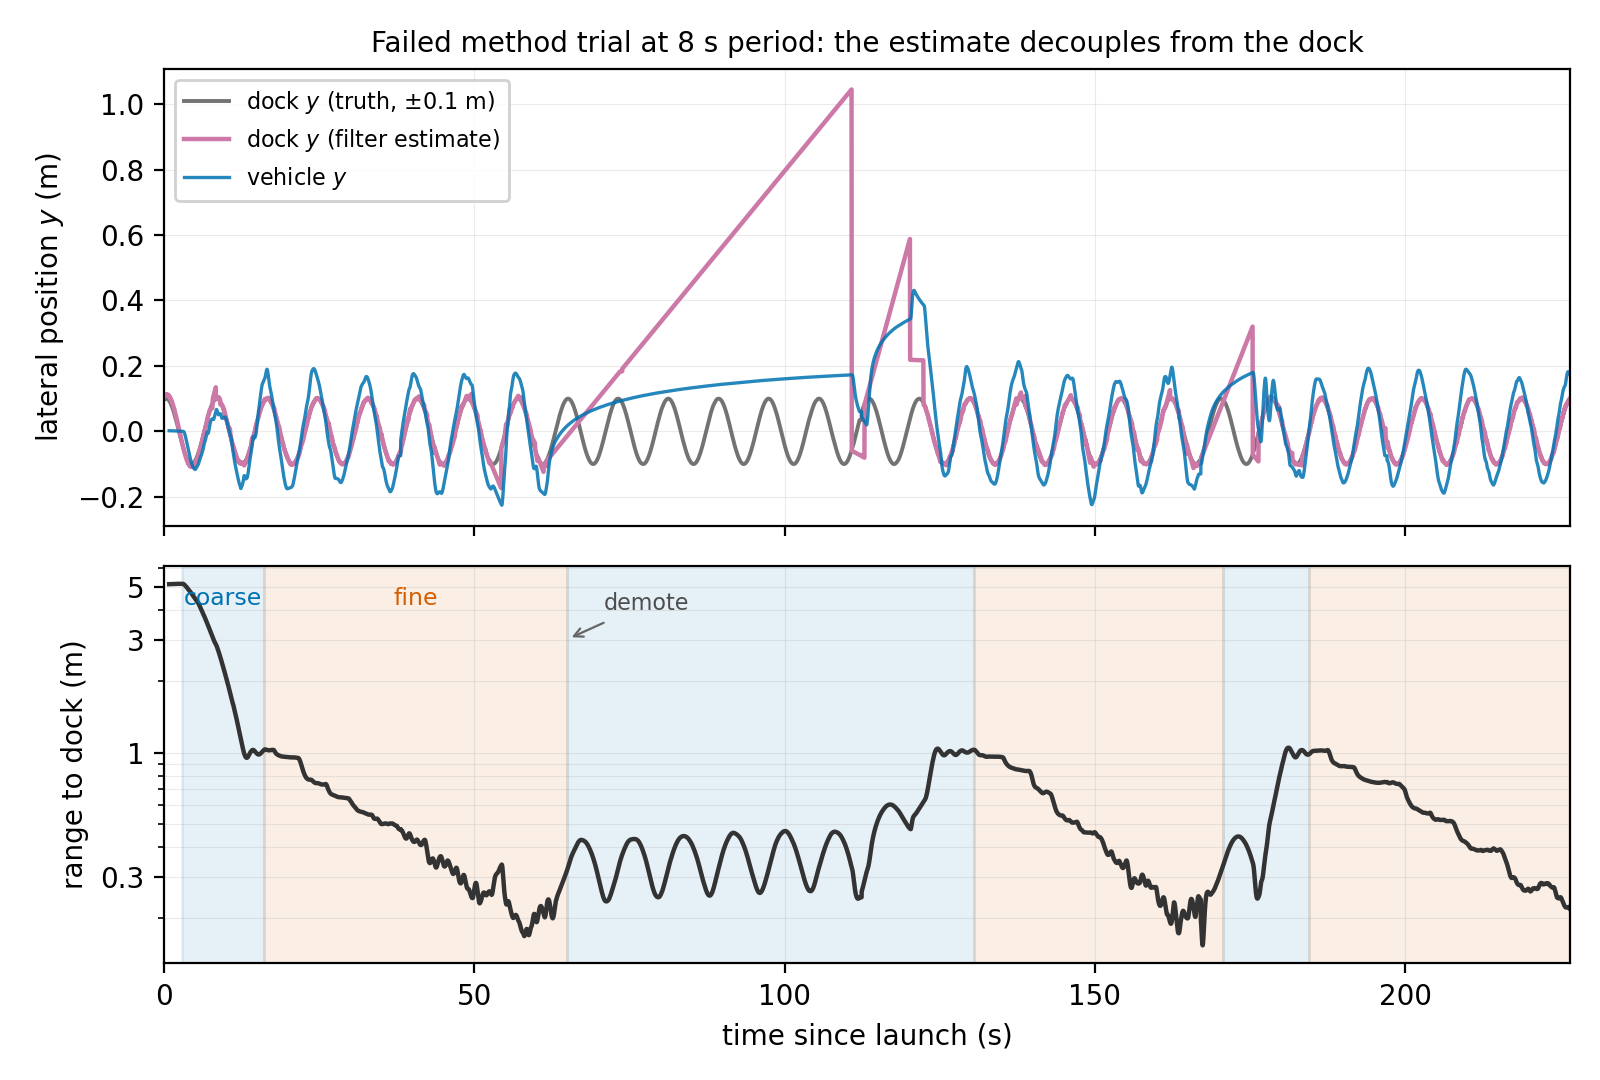
\includegraphics[width=0.75\textwidth]{Figures/rov_trajectory_failure.png}
    \caption{A failed method trial at the 8~s sway period. Top: lateral
        position of the true dock, the filter's dock estimate and the
        vehicle. Bottom: range to the dock with mission phases shaded.}
    \label{fig:trajectory-failure}
\end{figure}

This failure also hides itself from the system. Every alignment signal the system exposes is computed against its own estimate, and in the failed trials those signals read seat-tolerance alignment (lateral errors of 0.000 to 0.017~m) while the ground truth shows the vehicle 0.17 to 0.48~m off axis at the dock plane. Only the ground-truth channel exposes the divergence, which argues for independent verification in any real deployment.

Whether this failure would transfer to hardware depends on whether the 240~ms plant lag is real or a simulation artefact, since the loop-gain argument places the cliff where the lag becomes comparable to the sway timescale. The lag is not a compute artefact, since the sweep replicated at real-time factors of 0.6 and 1.0 with the cliff in the same place, so the lag does not scale with simulation load. Its origin is also not simulator-specific. The autopilot in the loop is the same ArduSub firmware a physical BlueROV2 runs, executed software-in-the-loop, so the path from velocity command through mode controller to motor mixing is the production code path. The remainder of the lag is the physics of accelerating the vehicle's inertia and added mass under bounded thrust, both taken from the vehicle's hydrodynamic model. If anything, the simulation is optimistic, since a real vehicle adds ESC and thruster response, the autopilot's own sensor filtering, and tether drag, none of which are modelled. The hardware lag should therefore be equal or larger, the instability would appear at the same or longer sway periods, and a hardware feedforward design cannot assume the lag away.

Three increasingly strong mitigations were evaluated. Bounding the velocity state at the physical dock speed and adding the covariance ceiling eliminated the metre-scale runaway and the resulting collisions, but did not restore fast-period docking. Sweeping the process noise density $\sigma_a$ over 0.02 to 0.16~m/s$^2$ found no stable setting, as the estimated amplitude remained 5 to 37 times the truth at every value, with no monotonic trend, because a smaller gain also makes the filter slower to shed an acquired phantom velocity. The baseline's immunity is therefore structural, and not a tuning point. Its velocity gain is zero by construction, and no finite gain reaches that property while the measurement error remains correlated with the vehicle motion. The conclusion is that dock velocity feedforward from a world-frame constant-velocity estimator requires explicit ego-motion compensation, by fusing vehicle odometry into the filter or by estimating in a vehicle-relative frame. This is identified as future work.

\subsubsection{Replication}

The sweep was run in full on two hosts (real-time factors 0.6 and 1.0) and two filter revisions (before and after the velocity bounds). The baseline's uniform success and the method's cliff between 10~s and 8~s reproduced in both, indicating that the result reflects the estimator design rather than compute load, hardware or incidental tuning.
